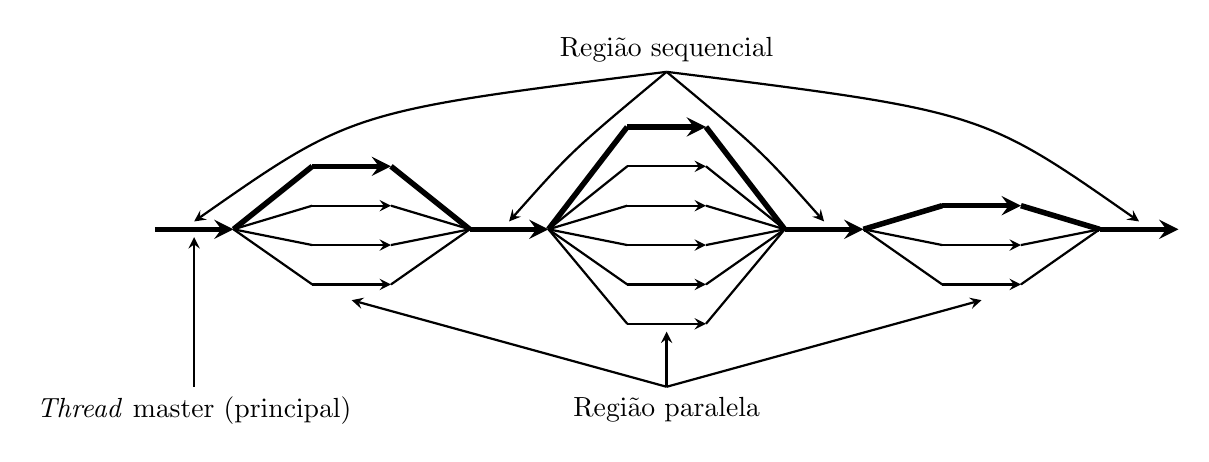
\begin{tikzpicture}[style=thick, >=stealth]%[line width=2pt]
\begin{scope}[line width=2pt]
  \draw[->] (0,0) -- (1,0);
  %
  \draw (1,0) -- (2,0.8);
  \draw[->] (2,0.8) -- (3,0.8);
  \draw (3,0.8) -- (4,0);
\end{scope}
%
\draw (1,0) -- (2,0.3);
\draw[->] (2,0.3) -- (3,0.3);
\draw (3,0.3) -- (4,0);
%
\draw (1,0) -- (2,-0.2);
\draw[->] (2,-0.2) -- (3,-0.2);
\draw (3,-0.2) -- (4,0);
%
\draw (1,0) -- (2,-0.7);
\draw[->] (2,-0.7) -- (3,-0.7);
\draw (3,-0.7) -- (4,0);
%
\begin{scope}[line width=2pt]
  \draw[->] (4,0) -- (5,0);
  %
  \draw (5,0) -- (6,1.3);
  \draw[->] (6,1.3) -- (7,1.3);
  \draw (7,1.3) -- (8,0);
\end{scope}
%
\draw (5,0) -- (6,0.8);
\draw[->] (6,0.8) -- (7,0.8);
\draw (7,0.8) -- (8,0);
%
\draw (5,0) -- (6,0.3);
\draw[->] (6,0.3) -- (7,0.3);
\draw (7,0.3) -- (8,0);
%
\draw (5,0) -- (6,-0.2);
\draw[->] (6,-0.2) -- (7,-0.2);
\draw (7,-0.2) -- (8,0);
%
\draw (5,0) -- (6,-0.7);
\draw[->] (6,-0.7) -- (7,-0.7);
\draw (7,-0.7) -- (8,0);
%
\draw (5,0) -- (6,-1.2);
\draw[->] (6,-1.2) -- (7,-1.2);
\draw (7,-1.2) -- (8,0);
%
\begin{scope}[line width=2pt]
  \draw[->] (8,0) -- (9,0);
  %
%  \draw (9,0) -- (10,0.8);
%  \draw[->] (10,0.8) -- (11,0.8);
%  \draw (11,0.8) -- (12,0);
\draw (9,0) -- (10,0.3);
\draw[->] (10,0.3) -- (11,0.3);
\draw (11,0.3) -- (12,0);
%
\end{scope}
%
\draw (9,0) -- (10,-0.2);
\draw[->] (10,-0.2) -- (11,-0.2);
\draw (11,-0.2) -- (12,0);
%
\draw (9,0) -- (10,-0.7);
\draw[->] (10,-0.7) -- (11,-0.7);
\draw (11,-0.7) -- (12,0);
%
\draw[->,line width=2pt] (12,0) -- (13,0);
%
\draw[<-] (2.5,-0.9) -- (6.5,-2) node[below] {Região paralela};
\draw[<-] (6.5,-1.3) -- (6.5,-2);
\draw[<-] (10.5,-0.9) -- (6.5,-2);
%
\draw[<-] (0.5,-0.1) -- (0.5,-2) node[below] {\textit{Thread} master (principal)};
%
\draw[<-] (4.5,0.1) ..  controls(5.3,1) .. (6.5,2) node[above] {Região sequencial};
\draw[<-] (0.5,0.1) .. controls(2.5,1.5) .. (6.5,2);
\draw[<-] (8.5,0.1) .. controls(7.7,1) .. (6.5,2);
\draw[<-] (12.5,0.1) .. controls(10.5,1.5) .. (6.5,2);
%
\end{tikzpicture}